\usetikzlibrary{positioning, quotes}
\item For\footnote{Source code on \url{https://github.com/jinhanloh2021/AI\_AS2}} the below graph (heuristic values are provided in red color and actual costs are in black
color), please provide answers to the following answers:\\
Please note that $S$ is start and $G$ is the goal state.
\begin{center}
  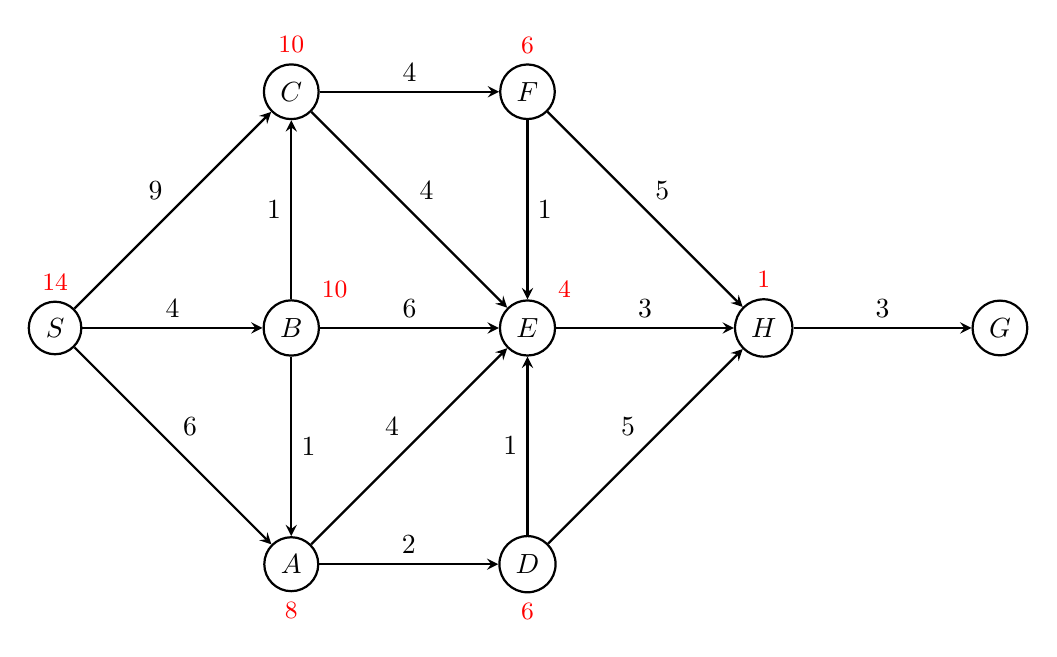
\begin{tikzpicture}[
      ->,>=stealth,auto,node distance=0cm,
      thick,main node/.style={circle,draw}
    ]
    \node[main node][label={[font=\small,text=red]above:$14$}] (S) at (0,3){$S$};
    \node[main node][label={[font=\small,text=red]below:$8$}] (A) at (3,0){$A$};
    \node[main node][label={[font=\small,text=red]above right:$10$}] (B) at (3,3){$B$};
    \node[main node][label={[font=\small,text=red]above:$10$}] (C) at (3,6){$C$};
    \node[main node][label={[font=\small,text=red]below:$6$}] (D) at (6,0){$D$};
    \node[main node][label={[font=\small,text=red]above right:$4$}] (E) at (6,3){$E$};
    \node[main node][label={[font=\small,text=red]above:$6$}] (F) at (6,6){$F$};
    \node[main node][label={[font=\small,text=red]above:$1$}] (H) at (9,3)  {$H$};
    \node[main node] (G) at (12,3){$G$};

    \draw [->]
    (S)  edge["6"] (A)
    (S)  edge["4"] (B)
    (S)  edge["9"] (C)
    (A)  edge["2"] (D)
    (B)  edge["6"] (E)
    (C)  edge["4"] (F)
    (B)  edge["1"] (A)
    (B)  edge["1"] (C)
    (A)  edge["4"] (E)
    (C)  edge["4"] (E)
    (F)  edge["1"] (E)
    (D)  edge["1"] (E)
    (D)  edge["5"] (H)
    (E)  edge["3"] (H)
    (F)  edge["5"] (H)
    (H)  edge["3"] (G);
  \end{tikzpicture}
\end{center}
\begin{enumerate}
  \item Is the heuristic admissible? Provide justification. Please fill in the intermediate table below to answer this question.
        \begin{center}
          \bgroup
          \def\arraystretch{1.5}%
          \captionsetup{type=figure}
          \begin{tabular}{|c|c|c|}
            \hline
            Node $n$ & Min cost to reach $G$ from $n$ & $h(n)$ \\
            \hline
            $S$      & $14$                           & $14$   \\
            $A$      & $9$                            & $8$    \\
            $B$      & $10$                           & $10$   \\
            $C$      & $10$                           & $10$   \\
            $D$      & $7$                            & $6$    \\
            $E$      & $6$                            & $4$    \\
            $F$      & $7$                            & $6$    \\
            $H$      & $3$                            & $1$    \\
            \hline
          \end{tabular}
          \captionof{table}{Comparison of min cost to goal and heuristic for every node}
          \egroup
        \end{center}
        Since $\forall n$, $h(n)\le Mincost(n)$, the heuristic $h$ is admissible.
  \item Is the heuristic consistent? Provide justification.\\[10pt]
        A heuristic is consistent if $\forall n \ \text{and}\  \forall p$, $h(n) \le c(n,p) + h(p)$. For the given graph, the heuristic $h$ is not consistent. This can be proven by counter-example.\\
        Take node $B$ and $A$. Given
        \begin{align*}
          h(B)   & = 10 \\
          c(B,A) & = 1  \\
          h(A)   & = 8  \\
        \end{align*}
        Then
        \begin{align*}
          h(B) & > c(B,A) + h(A) \\
          10   & > 8 + 1 = 9     \\
        \end{align*}
        Hence, $h$ is not consistent.
  \item Provide the search steps (as discussed in class) with vanilla \textbf{Breadth First Search (BFS)}. Show the \textbf{final solution path} and the \textbf{cost of that solution} for each algorithm. Also compute the search steps for \textbf{A* search} with the following heuristic:\\[10pt]
        Specify for each algorithm if the open list is queue, stack or priority queue. As a simplifying assumption, let index zero (i.e first element) in the open list be the top of the stack or front of the (priority) queue, as appropriate for the corresponding algorithm. Break ties by alphabetical order.\\
        Please use the following tables for your working. Open list contains nodes that are to be explored, and "nodes to add" are the successors of the node that is recently popped or dequeued.\\[10pt]
        \textbf{Breadth First Search algorithm}
        \begin{center}
          \bgroup
          \def\arraystretch{1.5}%
          \captionsetup{type=figure}
          \begin{tabular}{|c|c|c|c|}
            \hline
            Step \# & Open Queue           & Dequeue & Nodes to add \\
            \hline
            $1$     & $S$                  & $S$     & $A,B,C$      \\
            $2$     & $A^S, B^S, C^S$      & $A$     & $D,E$        \\
            $3$     & $B^S, C^S, D^A, E^A$ & $B$     &              \\
            $4$     & $C^S, D^A, E^A$      & $C$     & $F$          \\
            $5$     & $D^A, E^A, F^C$      & $D$     & $H$          \\
            $6$     & $E^A, F^C, H^D$      & $E$     &              \\
            $7$     & $F^C, H^D$           & $F$     &              \\
            $8$     & $H^D$                & $H$     & $G$          \\
            $9$     & $G^H$                & $G$     &              \\
            \hline
          \end{tabular}
          \captionof{table}{BFS priority queue}
          \egroup
        \end{center}
        Path taken is
        $$
          S \rightarrow A \rightarrow D \rightarrow H \rightarrow G
        $$
        \begin{align*}
          cost & = 6 + 2 + 5 + 3 \\
               & = 16
        \end{align*}
        \textbf{A* Search algorithm}\\
        Let $X^n_f$ be a node $X$, where $n$ is the parent state and $f=g(X) + h(X)$ as defined by the algorithm.
        \begin{center}
          \bgroup
          \def\arraystretch{1.5}%
          \captionsetup{type=figure}
          \begin{tabular}{|c|c|c|c|}
            \hline
            Step \# & Open Priority Queue                      & Dequeue & Nodes to add \\
            \hline
            $1$     & $S$                                      & $S$     & $A,B,C$      \\
            $2$     & $A^S_{14}, B^S_{14}, C^S_{19}$           & $A$     & $D,E$        \\
            $3$     & $B^S_{14}, D^A_{14}, E^A_{14}, C^S_{19}$ & $B$     & $A,C$        \\
            $4$     & $A^B_{13}, D^A_{14}, E^A_{14}, C^B_{15}$ & $A$     & $D,E$        \\
            $5$     & $D^A_{13}, E^A_{13}, C^B_{15}$           & $D$     & $E,H$        \\
            $6$     & $E^D_{12}, H^D_{13}, C^B_{15}$           & $E$     & $H$          \\
            $7$     & $H^E_{12}, C^B_{15}$                     & $H$     & $G$          \\
            $8$     & $G^H_{14}, C^B_{15}$                     & $G$     &              \\
            \hline
          \end{tabular}
          \captionof{table}{A* search priority queue}
          \egroup
        \end{center}
        Path taken is
        $$
          S \rightarrow B \rightarrow A \rightarrow D \rightarrow E \rightarrow H \rightarrow G
        $$
        \begin{align*}
          cost & = 4 + 1 + 2 + 1 + 3 + 3 \\
               & = 14
        \end{align*}
\end{enumerate}